\documentclass[border=8pt]{standalone}
\usepackage[utf8]{inputenc}
\usepackage[romanian]{babel}
\usepackage{tikz}
\usetikzlibrary{arrows.meta,positioning}

\begin{document}
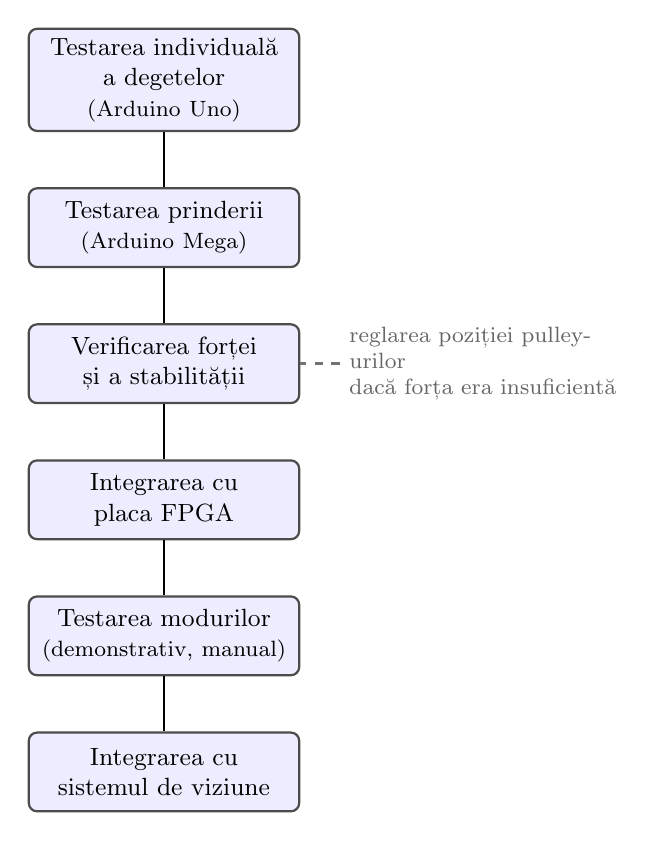
\begin{tikzpicture}[
  font=\small,
  >={Stealth[length=4pt]},
  stage/.style={draw=black!70,line width=0.8pt,rounded corners=3pt,
                minimum height=1.0cm,text width=3.2cm,align=center,fill=blue!7},
  lab/.style={font=\footnotesize,text=black!60},
  ->/.style={line width=1pt}
]

\node[stage] (s1) {Testarea individuală\\a degetelor\\\footnotesize(Arduino Uno)};
\node[stage,below=0.7cm of s1] (s2) {Testarea prinderii\\\footnotesize(Arduino Mega)};
\node[stage,below=0.7cm of s2] (s3) {Verificarea forței\\și a stabilității};
\node[stage,below=0.7cm of s3] (s4) {Integrarea cu\\placa FPGA};
\node[stage,below=0.7cm of s4] (s5) {Testarea modurilor\\\footnotesize(demonstrativ, manual)};
\node[stage,below=0.7cm of s5] (s6) {Integrarea cu\\sistemul de viziune};

\draw[->] (s1) -- (s2);
\draw[->] (s2) -- (s3);
\draw[->] (s3) -- (s4);
\draw[->] (s4) -- (s5);
\draw[->] (s5) -- (s6);

% eticheta laterala de reglaj la etapa de forta
\node[lab,right=0.5cm of s3,text width=3.6cm] (adj)
  {reglarea poziției pulley-urilor\\dacă forța era insuficientă};
\draw[->,dashed,black!55] (adj.west) -- (s3.east);

\end{tikzpicture}
\end{document}
